\documentclass[a4paper,12pt,oneside]{book}
\usepackage{polski}
\usepackage[utf8]{inputenc}
\usepackage{graphicx}
\graphicspath{{./images}}
\usepackage[shortlabels]{enumitem}
\usepackage{amssymb}
\usepackage{amsmath}
\usepackage{indentfirst}
\usepackage{pdfpages}

\usepackage{tikz}
%\usepackage{etoolbox} % for \ifthen
\usepackage{listofitems} % for \readlist to create arrays
\usetikzlibrary{arrows.meta} % for arrow size
\usepackage[outline]{contour} % glow around text
\contourlength{1.4pt}

\tikzset{>=latex} % for LaTeX arrow head
\usepackage{xcolor}
\colorlet{myred}{red!80!black}
\colorlet{myblue}{blue!80!black}
\colorlet{mygreen}{green!60!black}
\colorlet{myorange}{orange!70!red!60!black}
\colorlet{mydarkred}{red!30!black}
\colorlet{mydarkblue}{blue!40!black}
\colorlet{mydarkgreen}{green!30!black}
\tikzstyle{node}=[thick,circle,draw=myblue,minimum size=22,inner sep=0.5,outer sep=0.6]
\tikzstyle{node in}=[node,green!20!black,draw=mygreen!30!black,fill=mygreen!25]
\tikzstyle{node hidden}=[node,blue!20!black,draw=myblue!30!black,fill=myblue!20]
\tikzstyle{node convol}=[node,orange!20!black,draw=myorange!30!black,fill=myorange!20]
\tikzstyle{node out}=[node,red!20!black,draw=myred!30!black,fill=myred!20]
\tikzstyle{connect}=[thick,mydarkblue] %,line cap=round
\tikzstyle{connect arrow}=[-{Latex[length=4,width=3.5]},thick,mydarkblue,shorten <=0.5,shorten >=1]
\tikzset{ % node styles, numbered for easy mapping with \nstyle
	node 1/.style={node in},
	node 2/.style={node hidden},
	node 3/.style={node out},
}
\def\nstyle{int(\lay<\Nnodlen?min(2,\lay):3)} % map layer number onto 1, 2, or 3

\def\shrug{\texttt{\raisebox{0.75em}{\char`\_}\char`\\\char`\_\kern-0.5ex(\kern-0.25ex\raisebox{0.25ex}{\rotatebox{45}{\raisebox{-.75ex}"\kern-1.5ex\rotatebox{-90})}}\kern-0.5ex)\kern-0.5ex\char`\_/\raisebox{0.75em}{\char`\_}}}

\renewcommand\thechapter{\Roman{chapter}}
\renewcommand\thesection{\arabic{section}}
\renewcommand\thesubsection{\thesection.\arabic{subsection}}

\begin{document}

	
\includepdf{Odpowiedz-cover-page.pdf}

	\tableofcontents
	\newpage
	
	\chapter{Pytania - dr. hab. Bogdan Księżopolski}
	
		\section{Sieci i programowanie sieciowe}
			\subsection{Protokoły TCP i UDP - porównanie i zastosowanie.}
			
				\subsubsection*{TCP}
				
				Protokół TCP lub Transmission Control Protocol jest protokołem zorientowanym na połączenie, znajdującym się w warstwie transportowej modelu TCP / IP. Nawiązuje połączenie między komputerem źródłowym a docelowym przed rozpoczęciem komunikacji.
				
				\begin{figure}[h!]
					\centering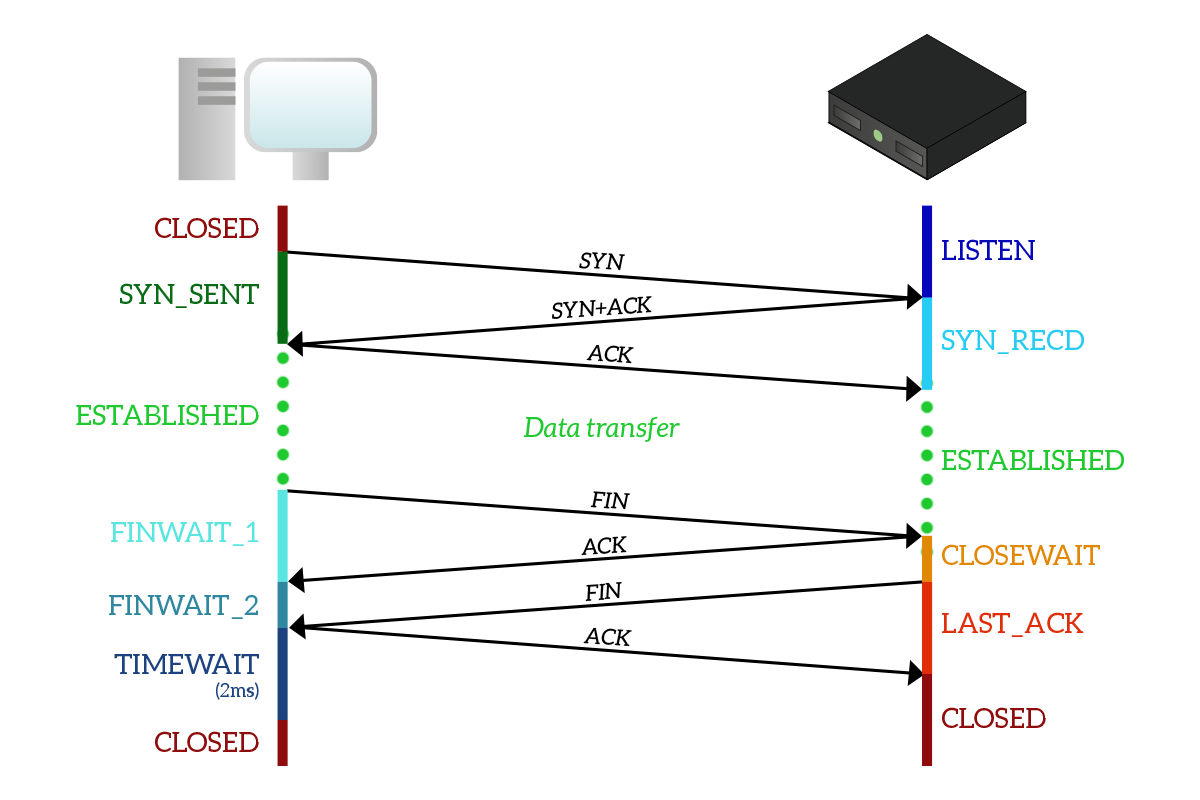
\includegraphics[scale=0.30]{tcp.png}
					\caption{TCP}
				\end{figure}
				
				Jest wysoce niezawodny, ponieważ wykorzystuje 3-drożną kontrolę uzgadniania, przepływu, błędu i przeciążenia. Zapewnia to, że dane wysyłane z komputera źródłowego są dokładnie odbierane przez komputer docelowy. Jeśli w przypadku, otrzymane dane nie są w odpowiednim formacie, to TCP ponownie przesyła dane.
				Poniższe protokoły używają TCP do transmisji danych:
				\begin{itemize}
					\item HTTP
					\item HTTPs
					\item FTP
					\item SMTP
				\end{itemize}
				
				\subsubsection*{UDP}
				
				\begin{figure}[h!]
					\centering
\includegraphics[scale=0.25]{udp.jpg}
					\caption{UDP :D}
				\end{figure}
				
				Protokół UDP lub User Datagram Protocol to bezpołączeniowy protokół znajdujący się w warstwie transportowej modelu TCP / IP. Nie ustanawia połączenia ani nie sprawdza, czy komputer docelowy jest gotowy do odbioru, czy też nie, po prostu przesyła dane bezpośrednio. Protokół UDP służy do przesyłania danych z większą szybkością. Jest mniej niezawodny i dlatego jest używany do przesyłania danych, takich jak pliki audio i wideo.
				UDP nie gwarantuje ani dostarczenia danych, ani nie przesyła utraconych pakietów.	
				
							
			
			\subsection{\color{red}Protokół IP.}
				rezerwuje - Rafał
			\subsection{\color{red}Modele sieci komputerowych.}
				a
			\subsection{\color{red}Porównanie protokołów IPv4 i IPv6.}
				a
			\subsection{\color{red}Format pakietu IP (poszczególne pola, zastosowanie).}
				rezerwuje - Rafał
			\subsection{\color{red}Ethernet.}
				a
			\subsection{\color{red}Protokoły warstwy aplikacji.}
				a
			\subsection{\color{red}Charakterystyka modelu OSI i TCP/IP.}
				rezerwuje - Rafał
			\subsection{\color{red}Rodzaje i przykłady nagłówków HTTP.}
				a
			\subsection{\color{red}Protokół WebSocket.}
				a
			\subsection{\color{red}Serwer zdarzeniowy, a wielowątkowy. Charakterystyka i porównanie.}
				a
		
		\section{Bezpieka}
			\subsection{\color{red}Infrastruktura klucza publicznego - charakterystyka.}
				a
			
			\subsection{Kryptografia symetryczna oraz asymetryczna - charakterystyka.}
				
				\subsubsection*{Kryptografia symetryczna}
				
				W kryptografii symetrycznej szyfrowanie i deszyfrowanie wykonywane jest przy użyciu tego samego klucza. W niektórych algorytmach wykorzystywane są dwa klucze, jednak muszą one być od siebie zależne w taki sposób, że znając jeden z nich, można wygenerować drugi.
				
				\begin{figure}[h!]
					\centering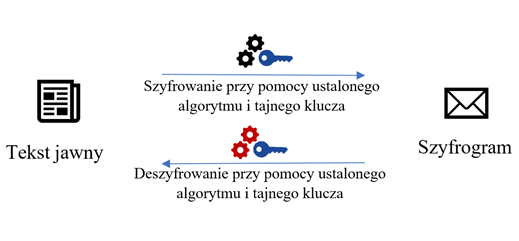
\includegraphics[scale=0.45]{krypt_sym.png}
					\caption{Zasada działania kryptografii symetrycznej}
				\end{figure}
				
				W celu zapewnienia bezpiecznej komunikacji, algorytm szyfrowania musi być tak skonstruowany, żeby odtworzenie tekstu jawnego bez znajomości klucza było zadaniem trudnym obliczeniowo. Dodatkowym wymaganiem jest tajność klucza – przed rozpoczęciem wymiany wiadomości, należy opracować protokół uzgadniania lub przekazywania klucza.
				
				Algorytmy szyfrowania symetrycznego możemy podzielić na algorytmy blokowe i strumieniowe. Pierwsze z nich przekształcają blok danych ustalonej długości, traktując go jako całość, na szyfrogram o tej samej liczbie bitów. Szyfry strumieniowe przyjmują natomiast ciąg (strumień) danych. Algorytmy kryptografii symetrycznej są szybkie, zwykle wymagają też mniejszej mocy obliczeniowej niż algorytmy asymetryczne. Powszechnie stosowanym szyfrem symetrycznych jest \textbf{AES}.
				
				\subsubsection*{Kryptografia asymetryczna}
				
				Kryptografia asymetryczna to rodzaj kryptografii, w którym jeden z używanych kluczy jest udostępniony publicznie. Każdy użytkownik może użyć tego klucza do zaszyfrowania wiadomości, ale tylko posiadacz drugiego, tajnego klucza może odszyfrować taką wiadomość.
				
				Kryptografia asymetryczna opiera się na funkcjach jednokierunkowych – takich, które da się łatwo wyliczyć w jedną stronę, ale bardzo trudno w drugą. Np. mnożenie jest łatwe, a rozkład na czynniki (z ang. faktoryzacja) trudny (na czym przykładowo opiera się \textbf{RSA}). Potęgowanie modulo jest łatwe, a logarytmowanie dyskretne jest trudne (na czym opierają się ElGamal, DSA i \textbf{ECC}).
				
				\begin{figure}[h]
					\centering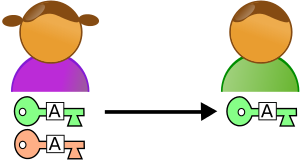
\includegraphics[scale=0.45]{krypt_asym_1.png}
					\caption{Krok 1: Alice przesyła do Boba swój klucz publiczny}
					
					\hspace{5pt}
					
					\centering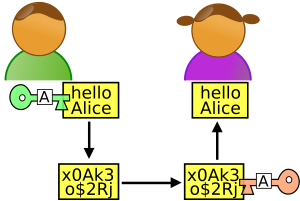
\includegraphics[scale=0.45]{krypt_asym_2.png}
					\caption{Kroki 2 i 3: Bob szyfruje wiadomość kluczem publicznym Alice, która to następnie otrzymuje zaszyfrowaną wiadomość i rozszyfrowuje ją kluczem prywatnym}
				\end{figure}
				
				Klucz publiczny używany jest do zaszyfrowania informacji, klucz prywatny do jej odczytu. Ponieważ klucz prywatny jest w wyłącznym posiadaniu adresata informacji, tylko on może ją odczytać. Natomiast klucz publiczny jest udostępniony każdemu, kto zechce zaszyfrować wiadomość.
				
				Ponieważ kryptografia asymetryczna jest o wiele wolniejsza od symetrycznej, prawie nigdy nie szyfruje się wiadomości za pomocą kryptosystemów asymetrycznych (również ze względu na ograniczenie wielkości szyfrowanej wiadomości). Zamiast tego szyfruje się jedynie klucz jakiegoś szyfru symetrycznego, takiego jak np. AES. Takie protokoły, łączące elementy kryptografii symetrycznej i asymetrycznej, nazywa się hybrydowymi.
				
				Nadawcy mogą także używać kluczy prywatnych do cyfrowego podpisywania wiadomości. Te podpisy cyfrowe pozwalają odbiorcom uwierzytelnić tożsamość nadawcy i spać spokojnie, wiedząc, że wiadomości nie zostały zmienione od momentu podpisania. W takim przypadku przesyłane informacje mogą być publiczne, a odbiorca może użyć certyfikatu, który towarzyszy tej informacji, aby zweryfikować integralność i autentyczność podpisanej wiadomości.
				
				\begin{figure}[h]
					\centering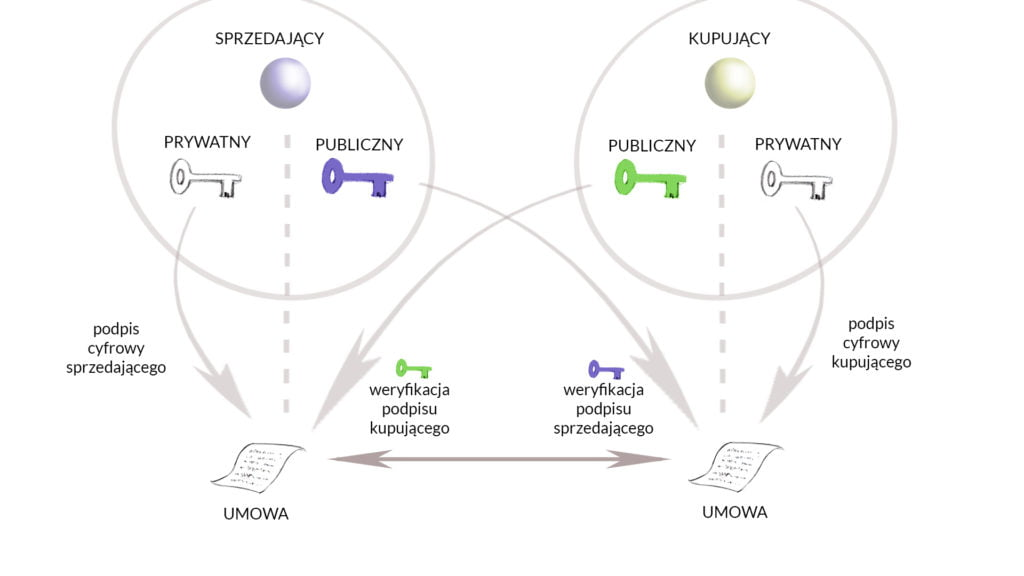
\includegraphics[scale=0.35]{krypt_asym_podpis.png}
					\caption{Jak działa podpis}
				\end{figure}
				
			\subsection{\color{red}Bezpieczeństwo sieci w odniesieniu do warstw modelu TCP/IP.}
				a
			\subsection{\color{red}Metody kontroli dostępu w systemach IT.}
				a
			\subsection{\color{red}Atrybuty bezpieczeństwa informacji.}
				a
	
	\chapter{Pytania - dr. hab. Grzegorz Wójcik}
	
		\section{Bazy danych}
			\subsection{\color{green} Paweł \color{red}Model relacyjny baz danych i języki zapytań.}
				a
			\subsection{\color{green} Paweł \color{red}Model obiektowo-relacyjny baz danych, inne modele danych.}
				a
			\subsection{\color{green} Paweł \color{red}Składnia podstawowych zapytań języka SQL.}
				a
			\subsection{\color{green} Paweł \color{red}Projektowanie baz danych oraz model związków encji.}
				a
			\subsection{\color{green} Paweł \color{red}Problemy indeksowania baz danych, rodzaje indeksów, indeksy typu B+ drzewo.}
				a
			\subsection{\color{green} Paweł \color{red}Przetwarzanie transakcyjne OLTP (On-Line Transaction Processing).}
				a
		
		\section{Paradygmaty}
			\subsection{\color{red}Założenia paradygmatu programowania obiektowego.}
				a
			\subsection{\color{red}Idea dziedziczenia i polimorfizmu w programowaniu.}
				a
			\subsection{\color{red}Zasady programowania dynamicznego.}
				a
			\subsection{\color{red}Główne paradygmaty programowania.}
				a
			\subsection{\color{red}Cechy programowania deklaratywnego.}
				a
	
	\chapter{Pytania - reszta}
	
		\section{Jezyk C i C++}
			\subsection{\color{red}Instrukcje sterujące w języku C.}
				a
			\subsection{\color{red}Zarządzanie pamięcią w języku C.}
				a
			\subsection{\color{red}Budowa, obsługa i formatowanie łańcuchów znakowych w języku C.}
				a
			\subsection{\color{red}Zasięg i czas życia obiektów w języku C++.}
				a
			\subsection{\color{red}Obsługa wyjątków w języku C++.}
				a
			\subsection{\color{red}Definicje obiektu, klasy i szablonu klasy w języku C++.}
				a
		
		\section{Algosy}
			\subsection{\color{red}Algorytmy sortujące.}
				a
			\subsection{\color{red}Algorytmy zachłanne.}
				a
			\subsection{\color{red}Metoda ,,dziel i zwyciężaj'' konstruowania algorytmów.}
				a
			\subsection{\color{red}Struktura kopców binarnych.}
				a
			\subsection{\color{red}Algorytmy wyszukiwania najkrótszej ścieżki w grafie.}
				a
			\subsection{\color{red}Sposoby implementacji słownika.}
				a
			\subsection{\color{red}Tablice mieszające.}
				a
			\subsection{\color{red}Algorytmy Monte Carlo oraz algorytmy Las Vegas.}
				a
			\subsection{\color{red}Metody rozwiązywania rekurencji. Rekurencje Flawiusza i wieża w Hanoi.}
				a
			\subsection{\color{red}Algorytmy Euklidesa. Algorytmy faktoryzacji.}
				a
			\subsection{\color{red}Metody reprezentacji grafów w komputerze.}
				a
			\subsection{\color{red}Droga i cykl Eulera. Droga i cykl Hamiltona.}
				a
			\subsection{\color{red}Drzewo spinające graf.}
				a
		
		\section{Teoria obliczalności czy coś}
			\subsection{\color{red}Pojęcia P, NP, NP-zupełne.}
				a
		
		\section{Automaty i inne takie}
			\subsection{\color{red}Deterministyczne i niedeterministyczne automaty skończone.}
				a
			\subsection{\color{red}Automaty z epsilon przejściami, wyrażenia regularne.}
				a
			\subsection{\color{red}Kompilacja: gramatyka bezkontekstowa, skaner, parser, błędy.}
				a
		
		\section{Podstawy komputera i systemy operacyjne}
			\subsection{\color{red}Systemy liczbowe i konwersje pomiędzy nimi.}
			
				a
				
			\subsection{Sposoby cyfrowej reprezentacji liczby całkowitej i rzeczywistej.}
			
				\subsubsection{Liczby całkowite}
				
				\subparagraph{Kod \text{ZM} (kod znak-moduł)}
				
				Sprawa w kodzie ZM jest w miarę prosta i klarowna. Najstarszy bit $b_{n-1}$ dla n-bitowej liczby jest bitem znaku i określa czy liczba jest dodatnia czy ujemna:
				\begin{itemize}
					\item 0 - liczba dodatnia,
					\item 1 - liczba ujemna.
				\end{itemize}
				
				Bity od $b_{n-1}$ do $b_0$ odpowiadają za kodowanie wartości samej liczby. Wzór na obliczenie wartości liczby zakodowanej w \textbf{ZM}:
				\begin{center}
					$L_{ZM} = (-1)^{b_{n-1}} \cdot (b_{n-2}2^{n-2} + ... + b_22^2 + b_12^1 + b_02^0)$
				\end{center}
				
				Przykładowe kodowanie liczby na ośmiu bitach w kodzie \textbf{ZM}:
				\begin{center}
					$26 \longrightarrow \textbf{0}0011010 $\\
					$-26 \longrightarrow \textbf{1}0011010 $
				\end{center}
				
				Proste, logiczne, fajne. Pytania, problemy? To jedziemy dalej.
				
				
				\subparagraph{Kod \textbf{U2} (kod uzupełnień do 2)}
				
				Tutaj sprawa się nieco komplikuje z zapisem liczb ujemnych. Bit $b_{n-1}$ ma wagę $-2^{n-1}$ co sprawia, że musimy bitowo tak jakby zapisać odwrotność liczby, którą chcemy reprezentować jako ujemna (i dodać 1, żeby się wszystko zgadzało). W zapisie liczb dodatnich zapis jest identyczny jak w \textbf{ZM} - na najstarszym bicie musimy tylko zachować $0$.
				
				Istnieje prosty algorytm konwersji na U2 z wykorzystaniem ZM:
				\begin{enumerate}
					\item Zapisać moduł liczby w ZM,
					\item Dokonać inwersji bitów (0 na 1 i 1 na 0),
					\item Zwiększ wynik dodając 1.
				\end{enumerate}
				
				Przykład z liczbą -27 na 8 bitach:
				
				\begin{tikzpicture}[x=2.2cm,y=1.4cm]
					\node[text width=5cm] at (0, 0)   (a) {Zapisujemy liczbę 27 w ZM};
					\node[text width=3cm] at (0.5, 1)   (b) {$00011011$};
					\draw [-to] (0,0.2) -- (0.2,0.7);
					\node[text width=3cm] at (2, 1)   (b) {$11100100$};
					\node[text width=3cm] at (3.5, 1)   (b) {$\textbf{11100101}$};
					
					\draw [-to] (0.7,1) -- (1.2,1);
					\draw [-to] (2.2,1) -- (2.7,1);
					
					\node[text width=5cm] at (2, 2)   (a) {Odwracamy bity};
					\draw [-to] (1.7,1.8) -- (1.7,1.2);
					
					\node[text width=5cm] at (3.9, 0)   (a) {Dodajemy 1};
					\draw [-to] (3.2,0.2) -- (3.2,0.7);
				\end{tikzpicture}
				
				\subsubsection{Liczby rzeczywiste}
				
				\subparagraph{Zapis stałopozycyjny}
				
				Do zapisu liczby stałoprzecinkowej przeznaczona jest z góry określona liczba bitów, a pozycję przecinka ustala się
				arbitralnie, w zależności od wymaganej dokładności, wolne bity uzupełniając zerami. Do reprezentacji liczb ze
				znakiem stosuje także kod U2.
				
				Liczba $6,25=110,01_{(2)}$ zapisana na 8 bitach gdy częśd ułamkowa zajmuje 3 najmłodsze bity, ma postać:
				\begin{center}
					\begin{tikzpicture}[x=2.2cm,y=1.4cm]	
						\node[text width=3cm] at (0, 0)   (b) {$\underbrace{00110}_{\text{część całkowita}}$};
						\node[text width=3cm] at (0.39, 0.42)   (b) {$\overbrace{010}^{\text{część ułamkowa}}$};
					\end{tikzpicture}
				\end{center}
				
				A w reprezentacji U2 będzie miała postać:
				
				\begin{center}
					$11001110$
				\end{center}
				
				Część całkowita liczby zachowuje się identycznie jak w przypadku zwykłych liczb całkowitych, natomiast bity w części ułamkowej posiadają wagi $2^{-1}$, $2^{-2}$, itd. - czyli $\frac{1}{2}$, $\frac{1}{4}$, ..., więc ilość bitów w części ułamkowej wpływa na precyzję zapisu.
				
				\subparagraph{Zapis zmiennopozycyjny}
				
				Liczba zmiennoprzecinkowa jest komputerową reprezentacją liczb rzeczywistych zapisanych w postaci wykładniczej
				o podstawie 2. Przykładowa notacja:
				
				\begin{center}
					$(-1)^Z \cdot M \cdot 2^C = (-1)^Z \cdot (1+m) \cdot 2^{c - BIAS}$
				\end{center}
				gdzie:
				\begin{description}
					\item[$(-1)^Z$] - znak liczby
					\item[$M=1+m$] - znormalizowana mantysa (liczba spełniająca warunek: $1 \leq M \leq 2$). Ponieważ przed przecinkiem stoi zawsze 1, więc można ją przedstawić w postaci $1+m$, gdzie \emph{m} jest liczbę ułamkową: $0 \leq m \leq 1$)
					\item[$C=c-BIAS$] - cecha (liczba całkowita), która dzięki zastosowaniu stałej BIAS pozwoli przedstawid cechę w postaci
					różnicy c-BIAS (c jest liczbą całkowitą dodatnią, tzw spolaryzowana cechę)
					\item[$BIAS$] - stała (liczba całkowita BIAS zależna od danej implementacji – rozwiązuje problem znaku cechy)
				\end{description}
				Kodujemy wyłącznie:
				\begin{description}
					\item[z] - bit znaku
					\item[m] - mantysę pomniejszoną o 1
					\item[c] - cechę przesuniętą o BIAS
				\end{description}
				
				Załóżmy, że operujemy następującym zmiennopozycyjnym formatem zapisu liczby rzeczywistej:
				\begin{itemize}
					\item na zapis przeznaczamy 16 bitów
					\item najstarszy bit ($b_{15}$) to bit znaku (będziemy stosowad kod ZM)
					\item kolejne 6 bitów ($b_{9}$-$b_{14}$) to mantysa
					\item pozostałe bity ($b_0$-$b_8$) są przeznaczone na zapis cechy i przyjmijmy, że BIAS=9
				\end{itemize}
				
				Przedstawimy liczbę +0,0224609375 w powyższym formacie. Naszą liczbę zapisujemy w systemie binarnym w
				postaci wykładniczej o podstawie 2, przesuwamy przecinek zapisując ją w notacji wykładniczej:
				
				\begin{center}
					$0,0224609375 = 0,0000010111_{(2)} = 1,0111_{(2)} \cdot 2^{-6}$
				\end{center}
				
				Z tego wynika, że:
				
				\begin{itemize}
					\item Znak: $(-1)^0$
					\item Mantysa: $1.\textbf{\underline{0111}}_2$
					\item Cecha: $-6 = 3-9 = 11_2 - BIAS$
				\end{itemize}
				
				Oto liczba 0,0224609375 zapisana w zadanym formacie:
				\begin{center}
					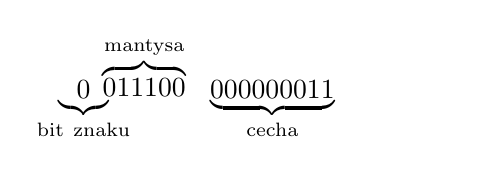
\begin{tikzpicture}[x=2.2cm,y=1.4cm]	
						\node[text width=3cm] at (0, 0)   (b) {$\underbrace{0}_{\text{bit znaku}}$};
						\node[text width=3cm] at (0.38, 0.39)   (b) {$\overbrace{011100}^{\text{mantysa}}$};
						\node[text width=3cm] at (1, 0)   (b) {$\underbrace{000000011}_{\text{cecha}}$};
					\end{tikzpicture}
				\end{center}
			
			\subsection{\color{red}Wielowarstwowa organizacja oprogramowania komputera.}
				a
			\subsection{\color{red}Procesy, zasoby i wątki.}
				a
			\subsection{\color{red}Planowanie przydziału procesora, priorytety, wywłaszczanie oraz planowanie.}
				a
			\subsection{\color{red}Zarządzanie pamięcią operacyjną.}
				a
			\subsection{\color{red}Problem zakleszczenia, algorytm Bankiera.}
				a
		
		\section{Inżynieria Oprogramowania}
			\subsection{\color{red}Standardowe metodyki procesu wytwórczego oprogramowania.}
				a
			\subsection{\color{red}Metodyki zwinne (agile).}
				a
			\subsection{\color{red}Metody testowania oprogramowania.}
				a
			\subsection{\color{red}Walidacja i weryfikacja oprogramowania.}
				a
			\subsection{\color{red}Diagramy UML (przypadków użycia, klas, aktywności, sekwencji, stanów, obiektów, wdrożenia).}
				a
			\subsection{\color{red}Wzorce projektowe programowania obiektowego.}
				a
			\subsection{\color{red}Wzorce architektoniczne.}
				a
		
		\section{Systemy wbudowane i elektronika}
			\subsection{\color{red}Różnice pomiędzy obsługą zdarzeń w przerwaniach sprzętowych a obsługą zdarzeń w pętli programowej.}
				a
			\subsection{\color{red}Stosowalność systemów opartych o mikrokontrolery vs stosowalność typowych komputerów (stacjonarnych i laptopów).}
				a
			\subsection{\color{red}Dekoder, multiplekser i demultiplekser: budowa, zasada, działania, przeznaczenie/zastosowanie.}
				a
			\subsection{\color{red}Podstawowe układy budujące system mikroprocesorowy i sposób wymiany informacji pomiędzy nimi.}
				a
\end{document}